\documentclass{article}

\usepackage[top=.75in, bottom=.75in]{geometry}

\usepackage{amsmath}
\usepackage{graphicx}
\usepackage{xcolor}

\begin{document}

\newcommand{\tda}[1]{\textcolor{red}{#1}}
\newcommand{\tdb}[1]{\textcolor{orange}{#1}}
\newcommand{\tdc}[1]{\textcolor{blue}{#1}}
\newcommand{\unk}[1]{\textcolor{red}{#1}}
\newcommand{\der}[1]{\textcolor{orange}{#1}}
\newcommand{\off}[2]{\textnormal{\emph{Off}}_{#1\rightarrow#2}}

\section*{Setup:} Assume 3 polypoint tags (A, B, C), all 1~m from each other.

\begin{itemize}
  \item $t_A$ = tx delay for tag A (unknown)
  \item $r_A$ = rx delay for tag A (unknown)
  \item $\lambda$ = time of flight for 1~m ($\lambda = \frac{1}{c}\times\textnormal{\texttt{DWT\_TIME\_UNITS}}$)
  \item $\epsilon$ = precise delay before sending the next packet (i.e.\ 5\,ms)
\end{itemize}

The goal is to determine the calibration factor for a tag, $cal_A = t_A + r_A$.

\section*{Protocol:}

The following sequence will recover the $cal_C$. Note that timestamps from
local clocks are not synchronized, nor can the clocks be assumed to be running
at exactly the same speed.

\bigskip

\noindent
\begin{minipage}{.35\textwidth}
  \begin{enumerate}
    \item Tag A sends a packet
    \item Tag C sends a packet after $\epsilon$
    \item Tag C sends a packet after $\epsilon$
  \end{enumerate}
\end{minipage}%
~~~~~%
\begin{minipage}{.65\textwidth}
  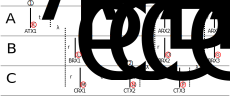
\includegraphics[width=\linewidth]{calibration_diagram}
\end{minipage}

\begin{align}
  BRX1 &= ATX1 + t_A + \lambda + r_B \\
  BRX2 &= ATX1 + t_A + \lambda + r_C + \epsilon_C + t_C + \lambda + r_B \\
  BRX2-BRX1 = \Delta_B &= r_C + t_C + \epsilon_C + \lambda \\
  ~\nonumber\\
  k_{C\rightarrow B} &= \frac{BRX3-BRX2}{CTX3-CTX2} \\
  ~\nonumber\\
  r_C + t_C &= \Delta_B - \epsilon_C \times k_{C\rightarrow B} - \lambda
\end{align}


\end{document}
